% Drawing 147/08-1 -- folder 147, batch 08, archive page 141 (PDF page 142).
% Transcription: À gauche du diagramme, un croquis : une bande courbe hachurée transversalement, marquée $V_{D'}$, autour d'une courbe $D'$ ; deux points de $D''$ sur $D'$, entourés chacun d'un petit disque hachuré, désignés par des flèches pointillées comme $V_{D''}$. Un numéro biffé (\struck{(2.35)}) au-dessus.
% Kind: tubular neighbourhood: hatched band with two hatched discs. Method 2 (schematic redraw from the facsimile). Status: ok.
% Notes: Beside the diagram, a sketch: a curved band hatched transversally, marked V_{D'}, round a curve D'; two points of D'' on D', each in a small hatched disc, pointed at by dotted arrows as V_{D''}. The struck number (2.35) above is drawn grey; the unstruck (2.35) of the formula is not part of the sketch.
% Coordinates: 1 unit = 1 mm = 1/100 of the crop width (bbox in page fractions: [0.076, 0.509, 0.434, 0.63]).
% Redrawn by Claude (claude-opus-5-5), issue #73, 2026-11-07; not checked by a human; not compiled (no TeX in the session).
% Rights: reproduces part of the work -- behind RENDER_TRANSCRIPTS, never published by itself.
\documentclass[tikz,border=3pt]{standalone}
\usepackage{amsmath,amssymb}
\usetikzlibrary{patterns,arrows.meta}
\tikzset{pencil/.style={black!45}, struck/.style={black!35}, mark/.style={circle,draw,inner sep=1.3pt}, pt/.style={circle,fill,inner sep=0.9pt}, opt/.style={circle,draw,fill=white,inner sep=1.1pt}}
\begin{document}
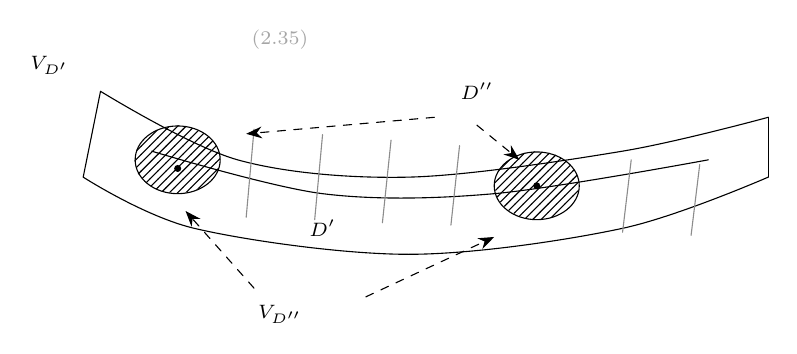
\begin{tikzpicture}[x=1mm,y=1mm,line cap=round,line join=round,font=\scriptsize]
\draw plot[smooth, tension=0.55] coordinates {(18.5,-21.2) (35.9,-29.9) (57.6,-32.1) (84.8,-28.8) (103.3,-24.5)};
\draw plot[smooth, tension=0.55] coordinates {(16.3,-32.1) (30.4,-38.6) (57.6,-41.9) (84.8,-38.6) (103.3,-32.1)};
\draw (18.5,-21.2) -- (16.3,-32.1);
\draw (103.3,-24.5) -- (103.3,-32.1);
\draw plot[smooth, tension=0.55] coordinates {(25,-28.8) (46.7,-34.2) (68.5,-34.2) (95.7,-29.9)};
\draw[pencil] (38,-26) -- (37,-37.2);
\draw[pencil] (46.7,-26.7) -- (45.7,-37.5);
\draw[pencil] (55.4,-27.4) -- (54.3,-37.9);
\draw[pencil] (64.1,-28.1) -- (63,-38.2);
\draw[pencil] (85.9,-29.9) -- (84.8,-39.1);
\draw[pencil] (94.6,-30.5) -- (93.5,-39.5);
\draw (28.3,-29.9) ellipse[x radius=5.4, y radius=4.3];
\fill[pattern=north east lines] (33.7,-29.9) -- (33.3,-31.6) -- (32.1,-33) -- (30.3,-33.9) -- (28.3,-34.2) -- (26.2,-33.9) -- (24.4,-33) -- (23.2,-31.6) -- (22.8,-29.9) -- (23.2,-28.2) -- (24.4,-26.8) -- (26.2,-25.9) -- (28.3,-25.5) -- (30.3,-25.9) -- (32.1,-26.8) -- (33.3,-28.2) -- cycle;
\node[pt] at (28.3,-31) {};
\draw (73.9,-33.2) ellipse[x radius=5.4, y radius=4.3];
\fill[pattern=north east lines] (79.3,-33.2) -- (78.9,-34.8) -- (77.8,-36.2) -- (76,-37.2) -- (73.9,-37.5) -- (71.8,-37.2) -- (70.1,-36.2) -- (68.9,-34.8) -- (68.5,-33.2) -- (68.9,-31.5) -- (70.1,-30.1) -- (71.8,-29.1) -- (73.9,-28.8) -- (76,-29.1) -- (77.8,-30.1) -- (78.9,-31.5) -- cycle;
\node[pt] at (73.9,-33.2) {};
\node[inner sep=1pt] at (12,-17.9) {\scriptsize $V_{D'}$};
\node[inner sep=1pt] at (46.7,-38.6) {\scriptsize $D'$};
\node[inner sep=1pt] at (66.3,-21.2) {\scriptsize $D''$};
\draw[dashed,-{Stealth[length=2mm]}] (60.9,-24.5) -- (37,-26.6);
\draw[dashed,-{Stealth[length=2mm]}] (66.3,-25.5) -- (71.7,-29.9);
\node[inner sep=1pt] at (41.3,-49.5) {\scriptsize $V_{D''}$};
\draw[dashed,-{Stealth[length=2mm]}] (38,-46.2) -- (29.3,-36.4);
\draw[dashed,-{Stealth[length=2mm]}] (52.2,-47.3) -- (68.5,-39.7);
\node[inner sep=1pt,struck] at (41.3,-14.7) {\scriptsize (2.35)};
\end{tikzpicture}
\end{document}
